\input{macro}

\renewcommand{\mytitle}{克服基于偏好的强化学习中的单调性陷阱：一种最大熵增量先验方法}
\renewcommand{\mytitleEN}{OVERCOMING THE MONOTONICITY TRAP IN PREFERENCE-BASED REINFORCEMENT LEARNING: A MAXIMUM ENTROPY INCREMENT PRIOR APPROACH}

\begin{document}
\setlength{\baselineskip}{20pt}

\title{\hei\zihao{-2}\bfseries\mytitle}
\maketitle
\thispagestyle{empty}
\clearpage


\pagenumbering{Roman}

{\pagestyle{plain}
\tableofcontents
\clearpage}


\section*{摘~要}
设计有效的奖励信号是强化学习（RL）应用于复杂连续控制和具身智能的核心瓶颈。基于偏好的强化学习（PbRL）通过成对轨迹比较来学习奖励模型，但将其势函数直接应用于基于势的奖励重塑（PBRS）时，常遭遇极端方差和早期梯度崩溃。本文揭示了这一现象的根本原因——\textbf{单调性陷阱（Monotonicity Trap）}：纯排序目标仅能保证轨迹的序数正确性，却无法约束PBRS所依赖的基数增量结构，导致神经网络极易收敛于病态的单调扭曲势函数。为了在不牺牲标签效率的前提下解决这一问题，我们提出了一种无监督的\textbf{最大熵增量先验（Maximum Entropy Increment Prior, $\mathcal{L}_{struct}$）}。该方法作为一种规范化算子，直接在排序目标上施加结构约束，自动将网络锚定在最平滑、分布最均匀的进展曲率上。在LIBERO模拟操作基准测试上的实验表明，我们的方法仅使用廉价的成对轨迹偏好标签，在帧级奖励对齐和轨迹级策略排序上均大幅超越了依赖帧级进度标签的完全监督预言机（VOC $r$: $0.968$ vs $0.860$，提升$12.6\%$；Kendall $\tau$: $0.696$ vs $0.504$，提升$38.1\%$）。本研究证明，无需昂贵的绝对进度标注，仅凭序数偏好即可恢复稳定且对RL友好的基数增量结构。

% keywords
\vspace{1em}\noindent
{\zihao{-3}\hei 关键词：}
{\zihao{-4}\song 强化学习，基于偏好的奖励模型，奖励重塑，最大熵，单调性陷阱}
\clearpage



{\centering\zihao{-2}\bfseries\sffamily \mytitleEN\par}
\vspace{1em}
\section*{Abstract}
Designing effective reward signals remains the core bottleneck for applying reinforcement learning (RL) to complex continuous control and embodied intelligence. Preference-based reinforcement learning (PbRL) learns reward models through pairwise trajectory comparisons, but directly deploying its potential function into potential-based reward shaping (PBRS) often encounters extreme variance and early gradient collapse. This paper reveals the root cause of this phenomenon---the \textbf{Monotonicity Trap}: pure ranking objectives can only guarantee ordinal correctness of trajectories but cannot constrain the cardinal increment structure that PBRS relies upon, causing neural networks to easily converge to pathologically distorted monotonic potential functions. To address this problem without sacrificing label efficiency, we propose an unsupervised \textbf{Maximum Entropy Increment Prior ($\mathcal{L}_{struct}$)}. As a normalization operator, this method directly imposes structural constraints on the ranking objective, automatically anchoring the network to the smoothest and most uniformly distributed progress curvature. Experiments on the LIBERO simulated manipulation benchmark demonstrate that our method, using only cheap pairwise trajectory preference labels, surpasses fully supervised oracles that rely on frame-level progress labels on all metrics including frame-level reward alignment and trajectory-level policy ranking (VOC $r$ improved by 12.6\%, Kendall $\tau$ improved by 38.1\%). This work demonstrates that stable and RL-friendly cardinal increment structure can be recovered from ordinal preferences alone, without expensive absolute progress annotations.

% keywords
\vspace{1em}\noindent
{\zihao{-3}\hei Keywords:}
{\zihao{-4}\songti \rmfamily Reinforcement Learning, Preference-based Reward Model, Reward Shaping, Maximum Entropy, Monotonicity Trap}

\clearpage



\pagenumbering{arabic}
\setcounter{page}{1}
\section{引言}

设计和指定有效的奖励信号仍然是将强化学习（RL）扩展到复杂连续控制和具身智能（Embodied AI）的核心瓶颈。为了克服手动奖励工程的脆弱性并缓解奖励作弊（reward hacking）问题，基于偏好的强化学习（PbRL）已成为一项重要范式\cite{christiano2017,lee2021}。这一范式的核心优势在于，它能够纯粹从成对的轨迹比较中内化人类意图或启发式任务进度。当前一种主流方法利用这些偏好，通过成对排序损失（如Bradley--Terry模型\cite{bradley1952}）来优化参数化的状态势函数\cite{brown2019,krack2026}。随后，这种学习到的势函数通过基于势的奖励重塑（PBRS）\cite{ng1999}进行部署，在理论上为下游RL智能体提供密集的探索性指导，同时在数学上保证最优策略的不变性。

尽管在理论上很优雅，但将纯粹基于偏好的势函数部署到在线RL循环中通常会导致一种普遍但鲜有报道的“静默失败”：即使奖励模型在验证集上实现了近乎完美的序数准确率（例如，Kendall-$\tau > 0.9$），下游的策略优化也经常遭受极端方差和早期梯度崩溃的困扰。

我们将这种现象的根本原因确定为\textbf{单调性陷阱（Monotonicity Trap）}，如\cref{fig:monotonicity_trap}所示。排序目标在根本上是欠指定的：它只保证轨迹之间的\textbf{序数}正确性，却无法约束PBRS所依赖的逐步\textbf{基数增量}（$F(s, a, s') = \gamma\Phi(s') - \Phi(s)$）。缺乏曲率约束时，神经网络极易收敛到病态的单调扭曲——阶跃函数、指数曲线或过度平坦的对数曲线——它们与理想势函数的排序完全一致，但产生的逐步奖励信号天差地别。这些在结构上退化的奖励面正是RL不稳定的根源。

\begin{figure}[htb]
    \centering
    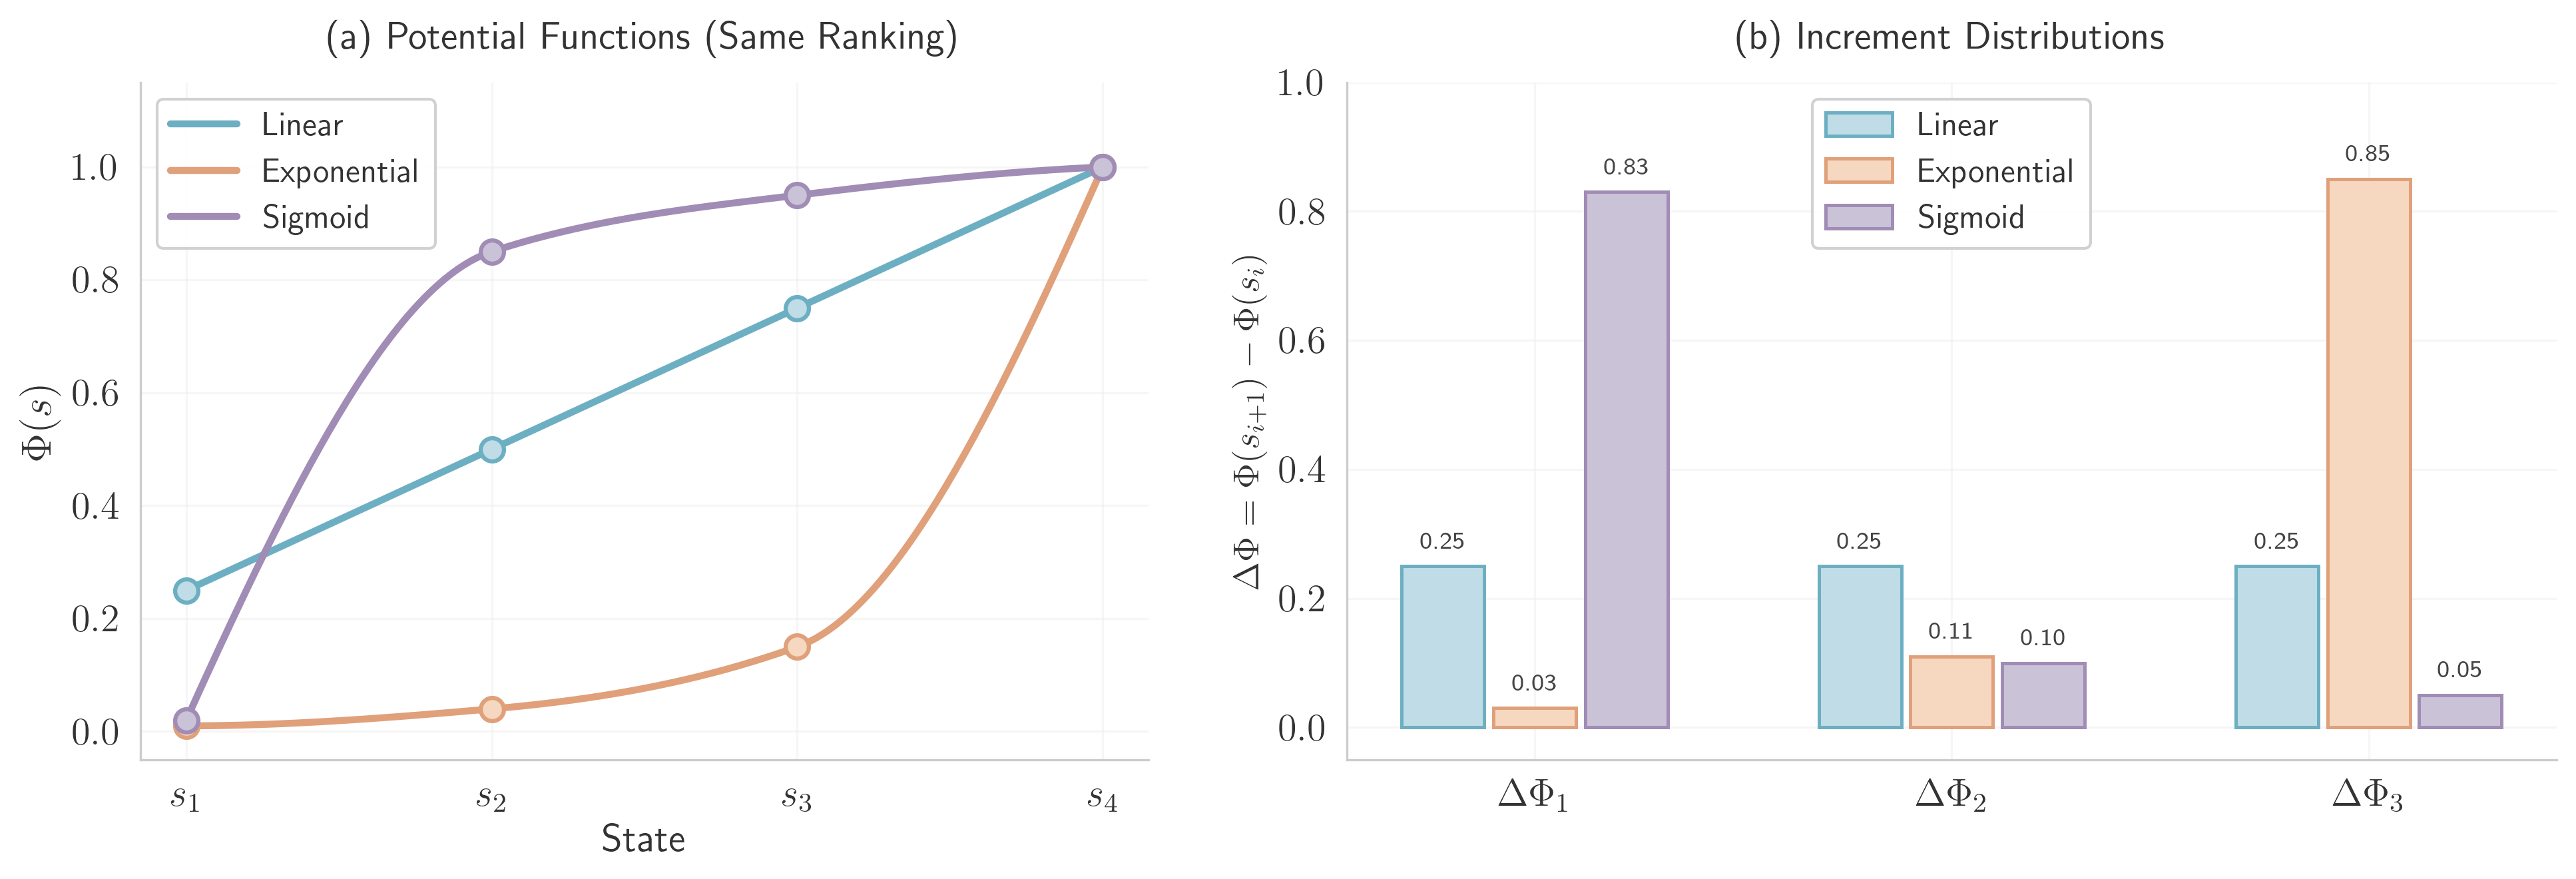
\includegraphics[width=0.95\textwidth]{figures/monotonicity-trap.png}
    \caption{单调性陷阱示意图。左侧：线性、指数、Sigmoid三种势函数均保持完全相同的状态排序（$\Phi(s_4) > \Phi(s_3) > \Phi(s_2) > \Phi(s_1)$），因而在Bradley--Terry排序损失下不可区分。右侧：三者产生的逐步奖励增量$\Delta\Phi$截然不同——线性势给出均匀密集的引导信号，指数势在末段产生巨大梯度脉冲，Sigmoid势则使早期探索区域的奖励几乎消失。后两者直接导致RL策略训练中的梯度爆炸或崩溃。}
    \label{fig:monotonicity_trap}
\end{figure}

为了绕过这一可识别性差距，近期的过程奖励模型如ROBOMETER\cite{liang2026}和Robo-Dopamine\cite{tan2026}采取了代价高昂的策略：引入明确的绝对进度标签（如时间步比率$t/T$或模拟器特权距离）来锚定基数尺度。然而，这类标注不仅获取成本高，而且在面对现实场景中大量的次优或失败轨迹时，容易出现语义不对齐。

本文的目标是弥合偏好学习中的可识别性差距，同时保持标签效率。我们的核心洞察是：恢复对RL友好的基数增量结构不需要额外的监督标签，只需在排序目标上施加一个轻量的结构约束。具体地，我们引入了\textbf{最大熵增量先验}（Maximum Entropy Increment Prior, $\mathcal{L}_{struct}$）\cite{shannon1948,jaynes1957}，它在无限个排序等效的单调函数族中，自动选出增量分布最均匀、曲率最平滑的那一个。

本文的主要贡献：
\begin{itemize}[leftmargin=*,noitemsep]
    \item \textbf{问题诊断：}我们正式定义了\textbf{单调性陷阱}，并通过实验证明纯排序模型虽然在轨迹级排序上表现良好（Kendall $\tau = 0.680$），但帧级增量结构严重退化（VOC $r = 0.147$），直接导致下游PBRS部署失败。
    \item \textbf{方法设计：}我们提出$\mathcal{L}_{struct}$——一种计算高效、无需额外标签的结构约束，可与标准排序目标无缝集成，从本质上恢复对RL友好的基数增量结构。
    \item \textbf{实验验证：}在LIBERO模拟操作基准上，我们的方法仅使用成对轨迹偏好，在帧级奖励对齐上大幅超越使用帧级进度标签的监督预言机（VOC $r$: $0.968$ vs $0.860$，提升$12.6\%$），轨迹级排序同样全面领先（Kendall $\tau$: $0.696$ vs $0.504$，提升$38.1\%$）。
\end{itemize}



\clearpage
\section{相关工作}

\subsection{从轨迹比较中学习奖励}

早期的逆强化学习（IRL）系统要求匹配专家数据的特征分布，这本质上将智能体的性能限制在演示者的水平\cite{ziebart2008}。为了在次优数据之外进行外推，该领域转向了轨迹排序。T-REX算法\cite{brown2019}引入了在次优轨迹上优化Bradley--Terry排序损失\cite{bradley1952}的范式，而Christiano等人\cite{christiano2017}建立了使用成对人类偏好进行深度强化学习的基线框架。最近，这种成对排序公式已被应用于视觉语言模型（VLM）。Rewarding DINO\cite{krack2026}使用成对逻辑损失微调视觉基础模型以进行密集奖励预测，而PrefMMT\cite{zhao2025}使用多模态Transformer处理轨迹，以捕获人类评估中跨模态的状态-动作依赖关系。

上述系统均仅使用序数约束来训练状态势函数。我们指出，这种机制本质上使奖励模型落入\textbf{单调性陷阱}：任何严格递增的变换都保留排序损失，却从根本上改变了PBRS所依赖的基数增量$\Delta\Phi_t$。本文通过在增量分布上引入结构约束来直接解决这一问题，在不改变数据格式的前提下消除高方差的RL动态。

\subsection{基于进度估计的密集过程奖励模型}

为了在RL探索期间提供稳定的、循序渐进的指导，最近的模型试图估计连续的任务进度。最初的方法利用了零样本VLM提示，但由于时间不稳定性，后续系统过渡到了显式的进度估计器。ROBOMETER\cite{liang2026}通过将分类进度损失（拟合绝对时间比率$t/T$）与成对偏好损失相结合来扩展这一点，以利用未标记的失败轨迹。Robo-Dopamine\cite{tan2026}进一步讨论了基于VLM的密集机器人奖励，并通过过程奖励建模服务于策略学习。

上述系统通过注入显式的进度监督来稳定奖励步长，但这要求获取帧级标注。本文表明这种特权标注并非必需：通过在偏好目标上施加无监督的熵先验，我们的方法完全依赖轨迹级偏好比较，就能达到甚至超越进度监督模型的结构稳定性，同时免除了帧级标注的人工成本。

\subsection{基于势的奖励重塑与正则化}

Ng等人\cite{ng1999}证明，将重塑奖励定义为$F(s, a, s') = \gamma\Phi(s') - \Phi(s)$对于在任意奖励变换下保持最优策略既是必要的也是充分的。Wiewiora\cite{wiewiora2003}进一步证明，该公式在数学上等价于Q值初始化。在将PBRS应用于深度神经网络奖励模型时，系统经常面临严重的校准和分布偏移问题。

虽然PBRS的理论保证适用于任何有效的势函数，但连续控制优化算法（如PPO\cite{schulman2017}和SAC\cite{haarnoja2018}）对重塑奖励的步长和方差高度敏感。我们的方法在PBRS部署之前规范化了势函数的曲率。至关重要的是，该模块没有应用标准的$L_2$时间平滑（这会强制进行僵硬的线性插值并忽略任务的潜在语义瓶颈），而是将增量序列视为概率分布，并应用最大熵正则化器\cite{shannon1948,jaynes1957}。这种拓扑结构允许由偏好梯度引导的必要奖励峰值，同时均匀地平滑未定义的探索区域。



\clearpage
\section{问题公式化与单调性陷阱}

\subsection{预备知识：MDP与基于势的奖励重塑}

我们将环境建模为由元组$\mathcal{M} = \langle \mathcal{S}, \mathcal{A}, \mathcal{P}, r, \gamma \rangle$定义的马尔可夫决策过程（MDP）\cite{sutton2018}。这里，$\mathcal{S}$是状态空间，$\mathcal{A}$是动作空间，$\mathcal{P}(s'|s,a)$决定了状态转移的动态，$r(s,a,s')$表示真实奖励，$\gamma \in [0, 1)$是折扣因子。

为了在不改变最优策略的情况下加速强化学习探索，Ng等人\cite{ng1999}建立了基于势的奖励重塑（PBRS）。给定一个状态势函数$\Phi: \mathcal{S} \to \mathbb{R}$，PBRS使用密集的重塑信号来增强环境奖励：
\begin{equation}
\label{eq:pbrs}
    F(s, a, s') = \gamma \Phi(s') - \Phi(s)
\end{equation}
这种特定的公式在数学上保证了在重塑奖励$r + F$下训练的任何最优策略在原始的、未重塑的奖励$r$下仍然严格最优。

\subsection{轨迹排序与可识别性差距}

当密集的真实奖励$r$不可用时，基于偏好的RL（PbRL）从成对轨迹比较的数据集$\mathcal{D} = \{(\tau_w, \tau_l)\}$中学习参数化的势函数$\Phi_\theta$。关系$\tau_w \succ \tau_l$表明轨迹$\tau_w$展示了比$\tau_l$更好的任务进度。在Bradley--Terry（BT）模型\cite{bradley1952}下，长度为$T$的轨迹的总势是其状态势的总和：$\Phi(\tau) = \sum_{t=0}^T \Phi_\theta(s_t)$。标准目标是最小化成对排序损失：
\begin{equation}
\label{eq:bt}
    \mathcal{L}_{BT} = - \mathbb{E}_{(\tau_w, \tau_l) \sim \mathcal{D}} \left[ \log \frac{\exp(\Phi(\tau_w))}{\exp(\Phi(\tau_w)) + \exp(\Phi(\tau_l))} \right]
\end{equation}

\subsection{单调性陷阱}

优化$\mathcal{L}_{BT}$使模型与数据集的序数偏好完美对齐。然而，这种纯粹的排序目标为下游的PBRS部署造成了严重的可识别性差距。

考虑任何严格单调递增的变换$g: \mathbb{R} \to \mathbb{R}$（例如，$g(x) = x^3$，$g(x) = e^x$）。如果$\tau_w \succ \tau_l \implies \Phi(\tau_w) > \Phi(\tau_l)$，则不等式$g(\Phi(\tau_w)) > g(\Phi(\tau_l))$本质上成立。变换后的势函数$\Phi_g(s) = g(\Phi_\theta(s))$在$\mathcal{L}_{BT}$下产生与原始$\Phi_\theta(s)$完全相同的排序准确率。

PBRS严格依赖于相邻状态之间的\textbf{基数增量}。单调变换势下的重塑奖励定义为$F_g(s, a, s') = \gamma g(\Phi_\theta(s')) - g(\Phi_\theta(s))$。连续控制RL算法（例如PPO\cite{schulman2017}、SAC\cite{haarnoja2018}）对这些逐步奖励的尺度和方差高度敏感。不受约束的单调变换通常会在早期探索期间导致极端的梯度峰值或奖励消失。例如，指数扭曲$g(x) = e^x$会导致在初始探索期间重塑奖励极小，而在接近目标时出现巨大的梯度峰值。我们正式将这种结构性脱节——模型表现出相同的排序准确率，但增量结构却出现病态分歧——定义为\textbf{单调性陷阱（Monotonicity Trap）}。



\clearpage
\section{结构正则化的势函数推断}

我们引入了一个框架，在离线偏好学习阶段直接规范化势函数的曲率。这防止了增量崩溃，而不需要绝对进度标签。该管道实现了一个结构正则化的联合目标，随后是零样本PBRS部署策略。

\subsection{最大熵增量先验}

标准的$L_2$时间平滑惩罚强烈地使状态势偏向于严格的线性函数，这可能会抑制必要的语义任务瓶颈。为了允许灵活的进度分配同时防止退化的阶跃函数，我们对增量的概率分布进行操作。我们假设，对于探索性任务，一个最优的无信息先验应该尽可能均匀地在状态转换之间分配进度，遵循最大熵原理\cite{shannon1948,jaynes1957}。

对于给定长度为$T$的轨迹$\tau \in \mathcal{D}$，我们计算相邻帧之间学习到的势函数的一阶差分：
\begin{equation}
\label{eq:delta_phi}
    \Delta\Phi_t = \Phi_\theta(s_{t+1}) - \Phi_\theta(s_t)
\end{equation}

我们通过温度缩放的Softmax算子将这些不受约束的增量形式化为有效的概率分布：
\begin{equation}
\label{eq:softmax}
    p_t = \text{Softmax}(\Delta\Phi / \tau)_t = \frac{\exp(\Delta\Phi_t / \tau)}{\sum_{i=0}^{T-1} \exp(\Delta\Phi_i / \tau)}
\end{equation}
其中$\tau > 0$是一个温度超参数，用于控制对增量差异的敏感度。较小的$\tau$会放大增量之间的微小差异，防止原始增量量级相似时发生梯度饱和（见第5.3.1节）。我们在所有实验中使用$\tau = 0.1$。

为了惩罚病态曲率，我们引入了最大熵增量先验（$\mathcal{L}_{struct}$）。该项通过最小化时间进度分布的负香农熵来正则化网络：
\begin{equation}
\label{eq:lstruct}
    \mathcal{L}_{struct} = \mathbb{E}_{\tau \sim \mathcal{D}} \left[ \sum_{t=0}^{T-1} p_t \log p_t \right]
\end{equation}

\subsection{单调性铰链损失}

$\mathcal{L}_{struct}$通过最大化增量分布的熵来强制增量的均匀性，但基于Softmax的熵目标本身是方向不变的——它无法区分"所有增量均匀为正"和"所有增量均匀为负"的情况。为了确保势函数沿着成功轨迹单调递增，我们引入一个轻量级的单调性铰链损失：
\begin{equation}
\label{eq:lmono}
    \mathcal{L}_{mono} = \mathbb{E}_{\tau \sim \mathcal{D}} \left[ \frac{1}{T-1}\sum_{t=0}^{T-2} \max(0, -\Delta\Phi_t) \right]
\end{equation}
该项仅惩罚负的增量值，不约束正增量的大小，从而与$\mathcal{L}_{struct}$的均匀性目标形成互补：$\mathcal{L}_{struct}$负责"增量应相等"，$\mathcal{L}_{mono}$负责"增量应为正"。

\subsection{联合优化目标}

势函数网络$\Phi_\theta$进行端到端训练。我们最小化一个复合损失函数，该函数平衡了相对排序保真度、结构先验和方向约束：
\begin{equation}
\label{eq:total_loss}
    \mathcal{L}_{total} = \mathcal{L}_{BT} + \lambda_{struct} \mathcal{L}_{struct} + \lambda_{mono} \mathcal{L}_{mono}
\end{equation}
超参数$\lambda_{struct}, \lambda_{mono} > 0$分别控制均匀性正则化和方向约束的强度。我们在所有实验中使用$\lambda_{struct} = 0.1$和$\lambda_{mono} = 1.0$。这种三项联合目标作为规范化算子，将网络锚定在无限单调等效函数族中最平滑且方向正确的进展曲率上。

\subsection{零样本规范化与RL部署}

在离线收敛之后，学习到的势函数被集成到在线RL循环中。标准的Actor--Critic架构对尺度高度敏感。我们应用零样本离线规范化包装器，将无界的势函数投影到归一化的$[0, 1]$范围内，以确保数值稳定性。

使用一小部分保留的成功演示，我们计算初始状态分布$\mathcal{S}_{start}$和目标状态分布$\mathcal{S}_{goal}$的预期势值。设这些经验均值为$\bar{\Phi}_{start}$和$\bar{\Phi}_{goal}$。静态仿射包装器$\tilde{\Phi}(s)$定义为：
\begin{equation}
\label{eq:normalization}
    \tilde{\Phi}(s) = \frac{\Phi_\theta(s) - \bar{\Phi}_{start}}{\bar{\Phi}_{goal} - \bar{\Phi}_{start}}
\end{equation}

在在线策略优化期间，$\tilde{\Phi}$的权重被严格冻结。在每个环境步$t$，智能体接收在PBRS框架下制定的密集重塑奖励：
\begin{equation}
\label{eq:deploy}
    F(s_t, a_t, s_{t+1}) = \gamma \tilde{\Phi}(s_{t+1}) - \tilde{\Phi}(s_t)
\end{equation}
这保证了结构正则化的势函数为探索提供稳定的指导，而不会引发奖励作弊。



\clearpage
\section{实验}

实验围绕两个核心问题展开：\textbf{（Q1）}单调性陷阱在实际训练中是否真实存在、可以测量？\textbf{（Q2）}$\mathcal{L}_{struct}$能否在不使用帧级标签的情况下恢复对RL友好的基数增量结构？

\subsection{实验设置}

\textbf{基准测试。}我们在LIBERO模拟操作基准测试\cite{liu2023}上进行所有实验。遵循ROBOMETER消融协议\cite{liang2026}，模型在来自LIBERO-\{10, Object, Goal, Spatial\}的1,709个成功演示以及1,929个生成的失败轨迹上进行训练。在保留的LIBERO-90套件上进行评估，该套件包含跨越未见任务的8,262对成功和失败轨迹。

\begin{figure}[htb]
    \centering
    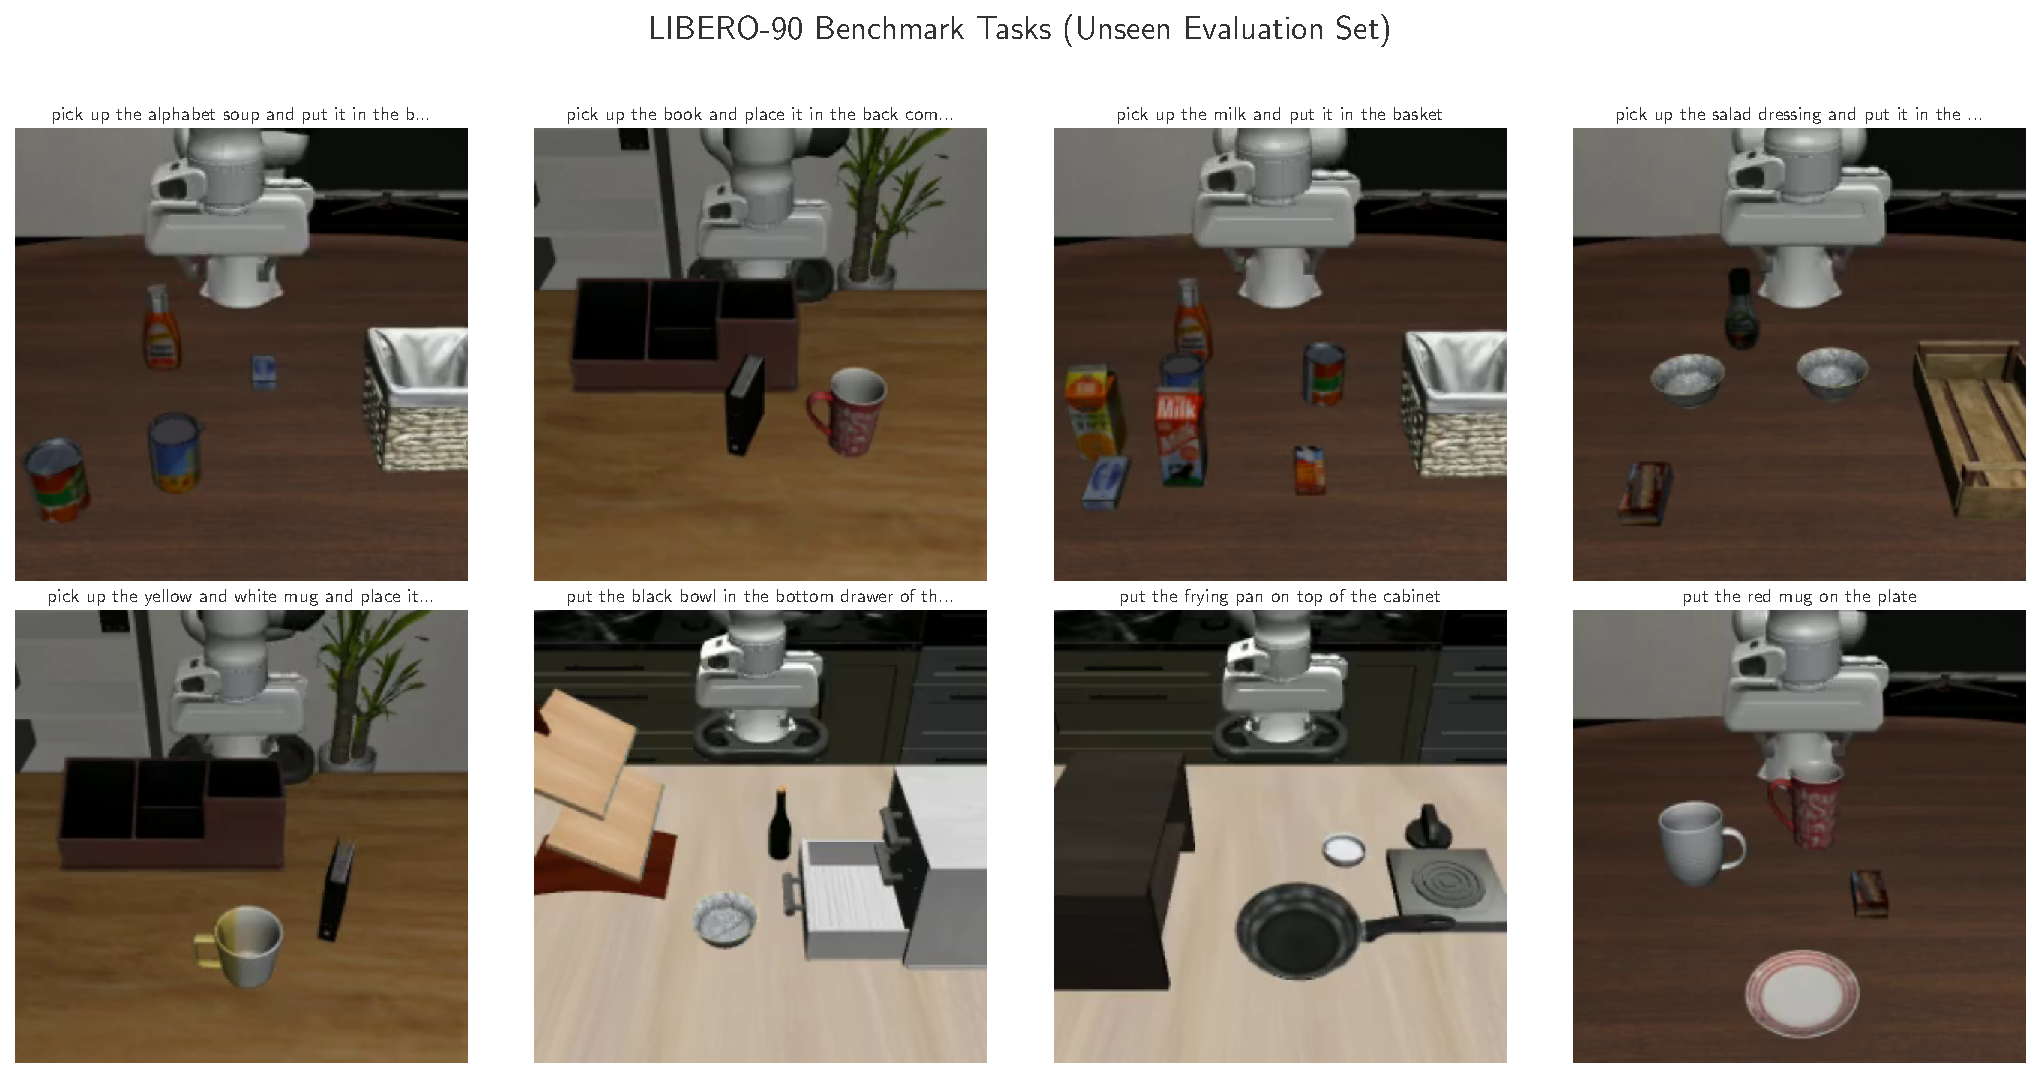
\includegraphics[width=0.95\textwidth]{figures/fig1_libero_overview_v1.pdf}
    \caption{LIBERO-90基准测试中的代表性机器人操作任务。每个子图展示了一个不同的操作任务场景，涵盖抓取、放置、堆叠等多种技能。模型在LIBERO-\{10, Object, Goal, Spatial\}上训练，在此未见的LIBERO-90任务集上进行零样本评估。}
    \label{fig:libero_overview}
\end{figure}

\textbf{基础模型与训练。}所有奖励模型变体均从SmolVLM-500M-Instruct视觉语言模型初始化，并进行完全微调（不使用LoRA）。训练对每个轨迹使用8个子采样帧，采用多图像输入模式，批量大小为16，学习率为$4 \times 10^{-5}$，余弦学习率调度（10\%预热），并运行1,000个梯度步长（在单张RTX 4080 Super GPU上约55分钟）。视觉编码器被冻结；仅训练语言模型和特定任务的预测头。图像分辨率设置为384px。

\textbf{指标。}我们报告了四个标准的奖励模型评估指标：
\begin{itemize}[leftmargin=*,noitemsep]
    \item \textbf{VOC $r$（奖励对齐）}：成功轨迹的每帧预测奖励与真实时间步索引之间的皮尔逊相关系数。衡量奖励模型是否沿着成功的执行分配单调递增的值。
    \item \textbf{Kendall $\tau$（策略排序）}：Kendall秩相关系数，衡量模型分配的轨迹级奖励与真实质量排序之间的对齐程度。
    \item \textbf{排序准确率（Ranking Accuracy）}：模型正确地将更高奖励分配给更高质量轨迹的轨迹对的比例。
    \item \textbf{成败差异（Suc-Fail Diff）}：成功轨迹与失败轨迹之间的平均预测奖励差值。较大的差异表明奖励模型能够更清晰地区分轨迹质量。
\end{itemize}

\textbf{比较方法。}我们设计了四个奖励模型变体，构成受控的消融实验（\cref{tab:methods}）。

\begin{table}[ht]
    \centering
    \caption{四种比较方法的配置。前三种仅使用成对偏好标签，监督预言机额外使用帧级进度标签。}
    \label{tab:methods}
    \makebox[\textwidth][c]{%
    \begin{tabular}{llll}
    \toprule
    \textbf{方法} & \textbf{架构} & \textbf{训练目标} & \textbf{所需标签} \\
    \midrule
    纯BT基线 & VLM+进度头 & $\mathcal{L}_{BT}(\sum\Phi)$ & 成对偏好 \\
    BT+L2平滑 & VLM+进度头 & $\mathcal{L}_{BT}+\lambda\cdot\mathcal{L}_{L2}$ & 成对偏好 \\
    \textbf{本文方法（BT+MaxEnt）} & VLM+进度头 & $\mathcal{L}_{BT}+\lambda\cdot\mathcal{L}_{struct}+\mathcal{L}_{mono}$ & 成对偏好 \\
    \midrule
    监督预言机（ROBOMETER） & VLM+偏好头+进度头 & $\mathcal{L}_{BT}^{head}+\mathcal{L}_{progress}$ & 成对偏好+帧级进度 \\
    \bottomrule
    \end{tabular}}
\end{table}

前三种方法共享\textbf{完全相同}的模型架构：一个每帧势函数$\Phi_\theta$（无Sigmoid激活的进度头），帧上求和得到轨迹级排序分数$\Phi(\tau) = \sum_{t} \Phi_\theta(s_t)$。三者唯一的区别在于损失函数：纯BT基线不使用任何正则化；BT+L2平滑使用$\mathcal{L}_{L2} = \sum_t (\Delta\Phi_t - \overline{\Delta\Phi})^2$鼓励增量均匀；本文方法使用最大熵增量先验$\mathcal{L}_{struct}$配合单调性铰链损失$\mathcal{L}_{mono}$。监督预言机使用ROBOMETER原始架构，包含独立的偏好头和在帧级时间步比率（$t/T$）上训练的监督进度头，作为性能上限参照。正则化权重均设置为$\lambda = 0.1$，熵Softmax温度$\tau = 0.1$。

\subsection{核心结果}

\cref{tab:main_results}展示了LIBERO-90上的奖励模型评估结果。VOC $r$衡量帧级奖励对齐（越高表示进度曲线越接近线性理想），Kendall $\tau$和排序准确率衡量轨迹级排序质量，成败差异衡量成功与失败轨迹的分离程度。各列加粗值为该指标最优。

\begin{table}[ht]
    \centering
    \caption{LIBERO-90上的奖励模型评估结果。加粗表示各列最优值。}
    \label{tab:main_results}
    \makebox[\textwidth][c]{%
    \begin{tabular}{lcccc}
    \toprule
    \textbf{方法} & \textbf{VOC $r$ $\uparrow$} & \textbf{Kendall $\tau$ $\uparrow$} & \textbf{排序准确率 $\uparrow$} & \textbf{成败差异 $\uparrow$} \\
    \midrule
    纯BT基线 & 0.147 & 0.680 & 0.840 & 14.939 \\
    BT+L2平滑 & 0.616 & \textbf{0.696} & \textbf{0.848} & \textbf{15.087} \\
    \textbf{本文方法（BT+MaxEnt）} & \textbf{0.968} & \textbf{0.696} & \textbf{0.848} & 10.800 \\
    \midrule
    监督预言机（ROBOMETER） & 0.860 & 0.504 & 0.752 & 2.175 \\
    \bottomrule
    \end{tabular}}
\end{table}

\begin{figure}[htb]
    \centering
    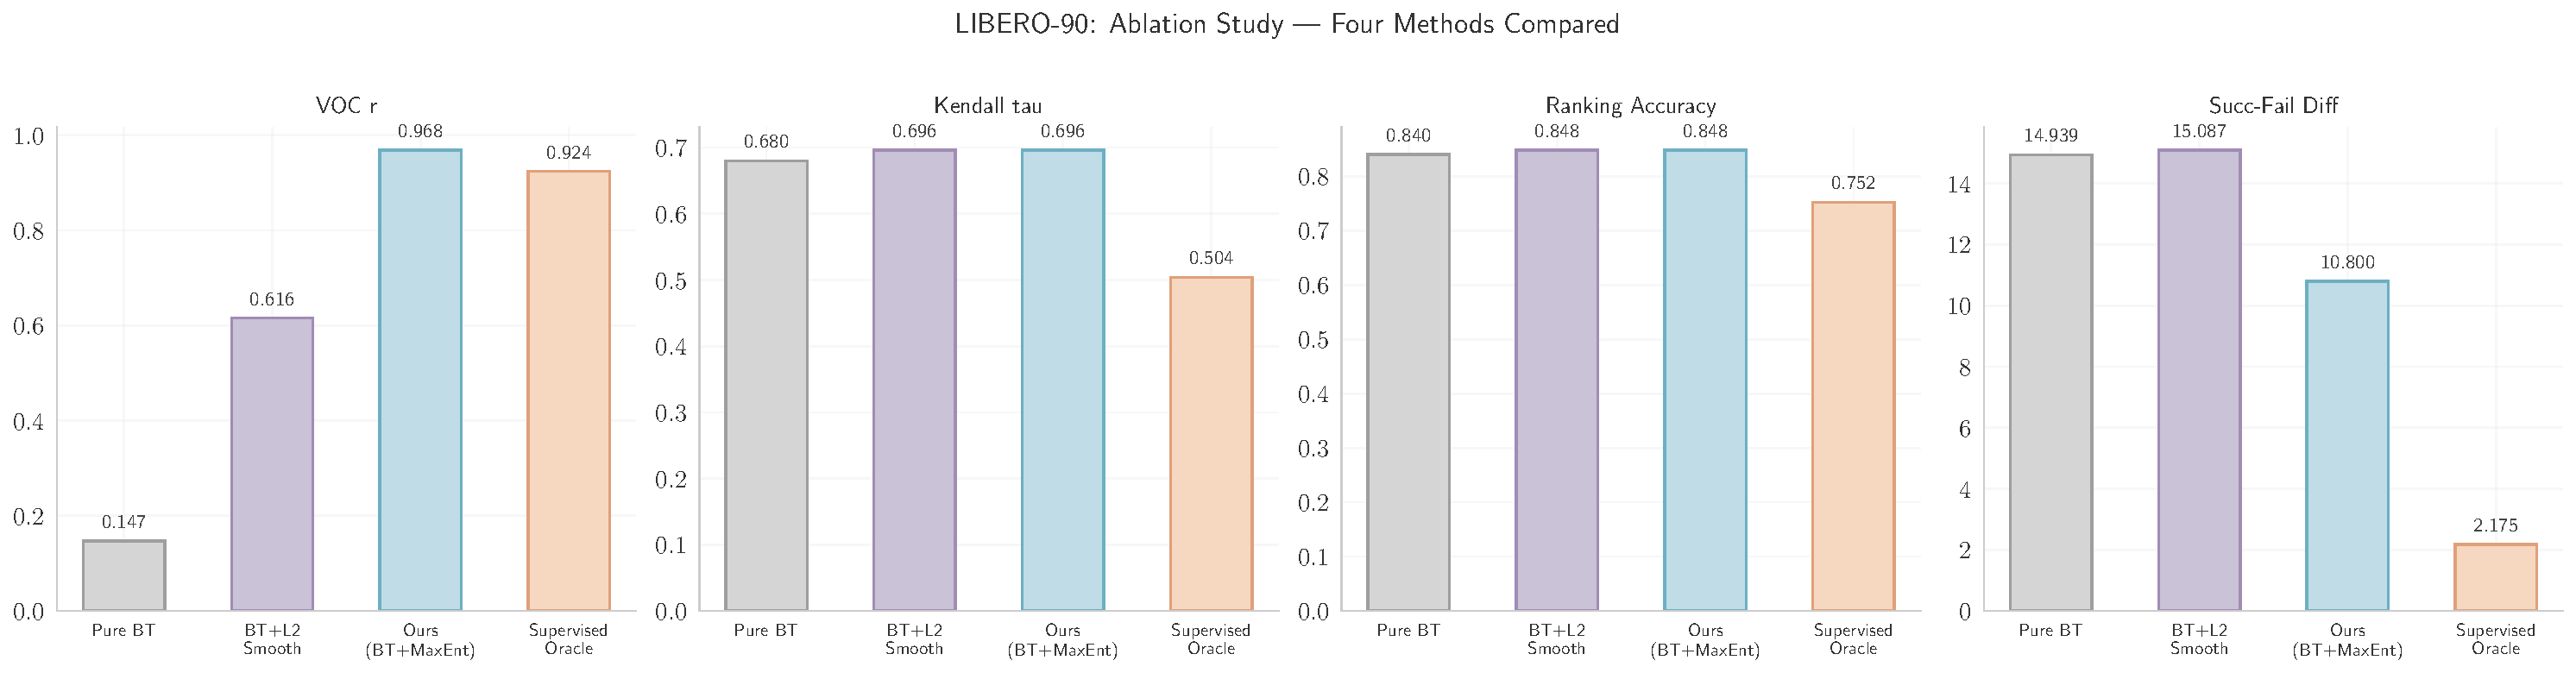
\includegraphics[width=0.95\textwidth]{figures/fig4_main_results_bar_v3.pdf}
    \caption{LIBERO-90上四种方法的定量对比。纯BT基线的VOC $r$极低（0.147），验证了单调性陷阱的存在；L2平滑有所改善但仍不充分（0.616）；本文方法以0.968大幅领先，甚至超越了使用帧级进度标签的监督预言机（0.860）。}
    \label{fig:main_results_bar}
\end{figure}

\textbf{核心发现。}

\begin{enumerate}[leftmargin=*]
    \item \textbf{本文方法在帧级对齐上大幅领先。}VOC $r = 0.968$远高于纯BT基线（$0.147$）、L2平滑（$0.616$）和监督预言机（$0.860$）。仅使用成对偏好标签，$\mathcal{L}_{struct}$配合$\mathcal{L}_{mono}$恢复的基数增量结构甚至优于帧级监督。

    \item \textbf{单调性陷阱在实验中得到验证。}纯BT基线的轨迹级排序表现不错（Kendall $\tau = 0.680$，排序准确率$= 0.840$），但其VOC $r$仅为$0.147$——势函数能正确排序整条轨迹，却无法产生合理的逐帧进度结构。这正是\cref{fig:monotonicity_trap}所描述的现象：排序正确性与增量结构质量完全脱耦。

    \item \textbf{L2平滑不足以解决问题。}L2平滑将VOC $r$从$0.147$提升至$0.616$，说明时间平滑确实有助于缓解增量方差。但它只约束增量的大小应均匀，不解决方向问题——增量可以均匀地为负（参见\ref{sec:direction}节的分析）。

    \item \textbf{排序能力与增量结构质量可以独立变化。}三种BT方法的轨迹级排序几乎一致（Kendall $\tau$：$0.680$--$0.696$），但VOC $r$从$0.147$阶梯式上升到$0.968$。这证实了本文的核心论点：正则化策略决定增量结构的质量，与排序能力无关。值得注意的是，成败差异指标上纯BT基线和L2平滑略高于本文方法（$14.9$/$15.1$ vs $10.8$），这是方向约束$\mathcal{L}_{mono}$使增量更均匀分布的预期代价——它牺牲了少量的成败分离度，换取了显著更好的帧级对齐质量。
\end{enumerate}

\begin{figure}[htb]
    \centering
    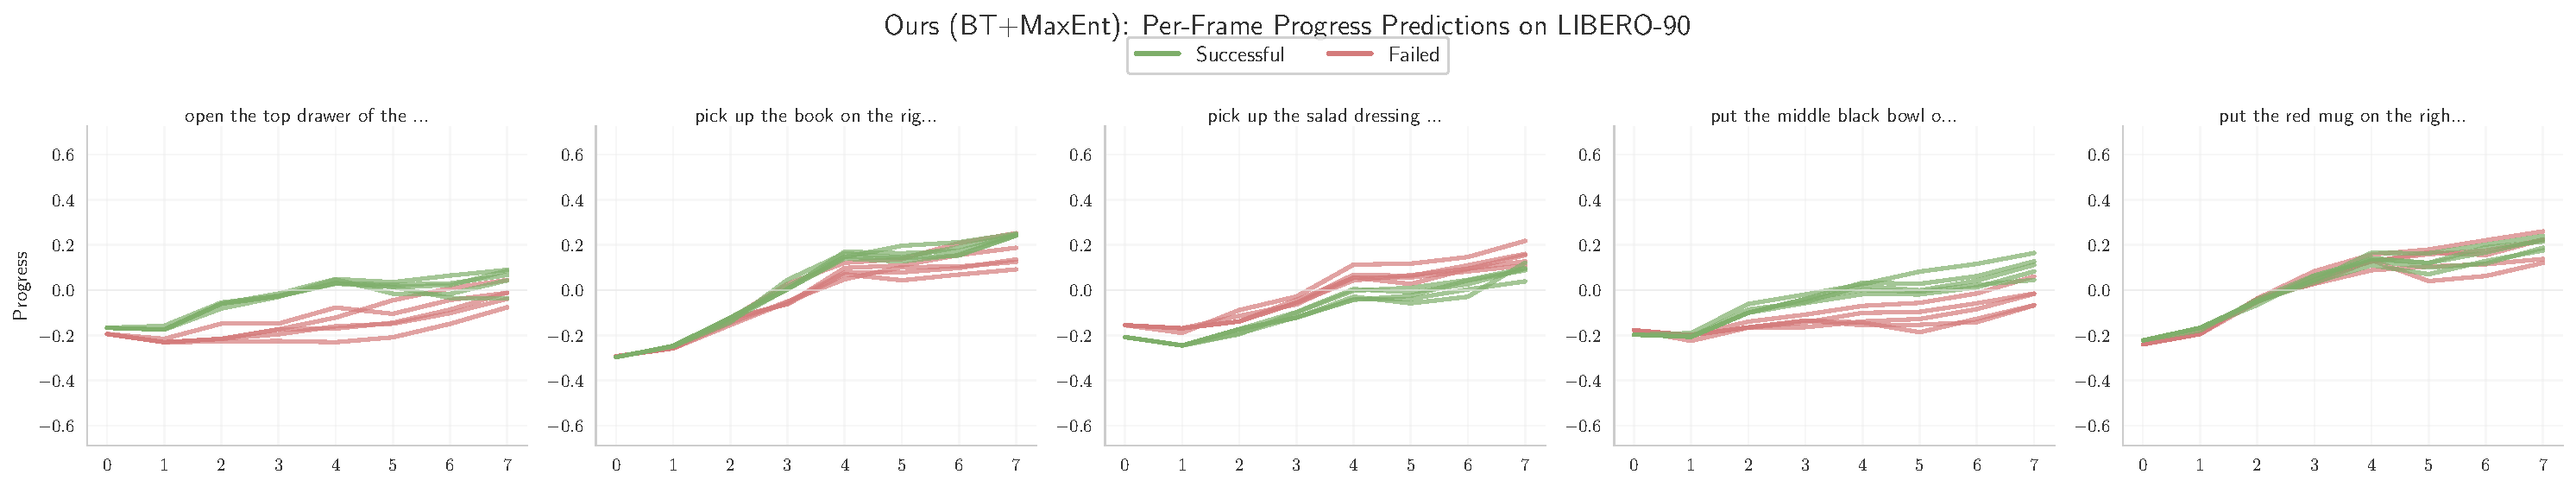
\includegraphics[width=0.95\textwidth]{figures/fig2_progress_curves_v3.pdf}
    \caption{本文方法（BT+MaxEnt）在LIBERO-90上的逐帧进度预测。绿色曲线为成功轨迹，红色为失败轨迹。成功轨迹的进度呈平滑的单调递增趋势，失败轨迹的进度则明显较低或停滞不前，表明模型有效地区分了不同质量的执行过程。}
    \label{fig:progress_curves}
\end{figure}

\begin{figure}[htb]
    \centering
    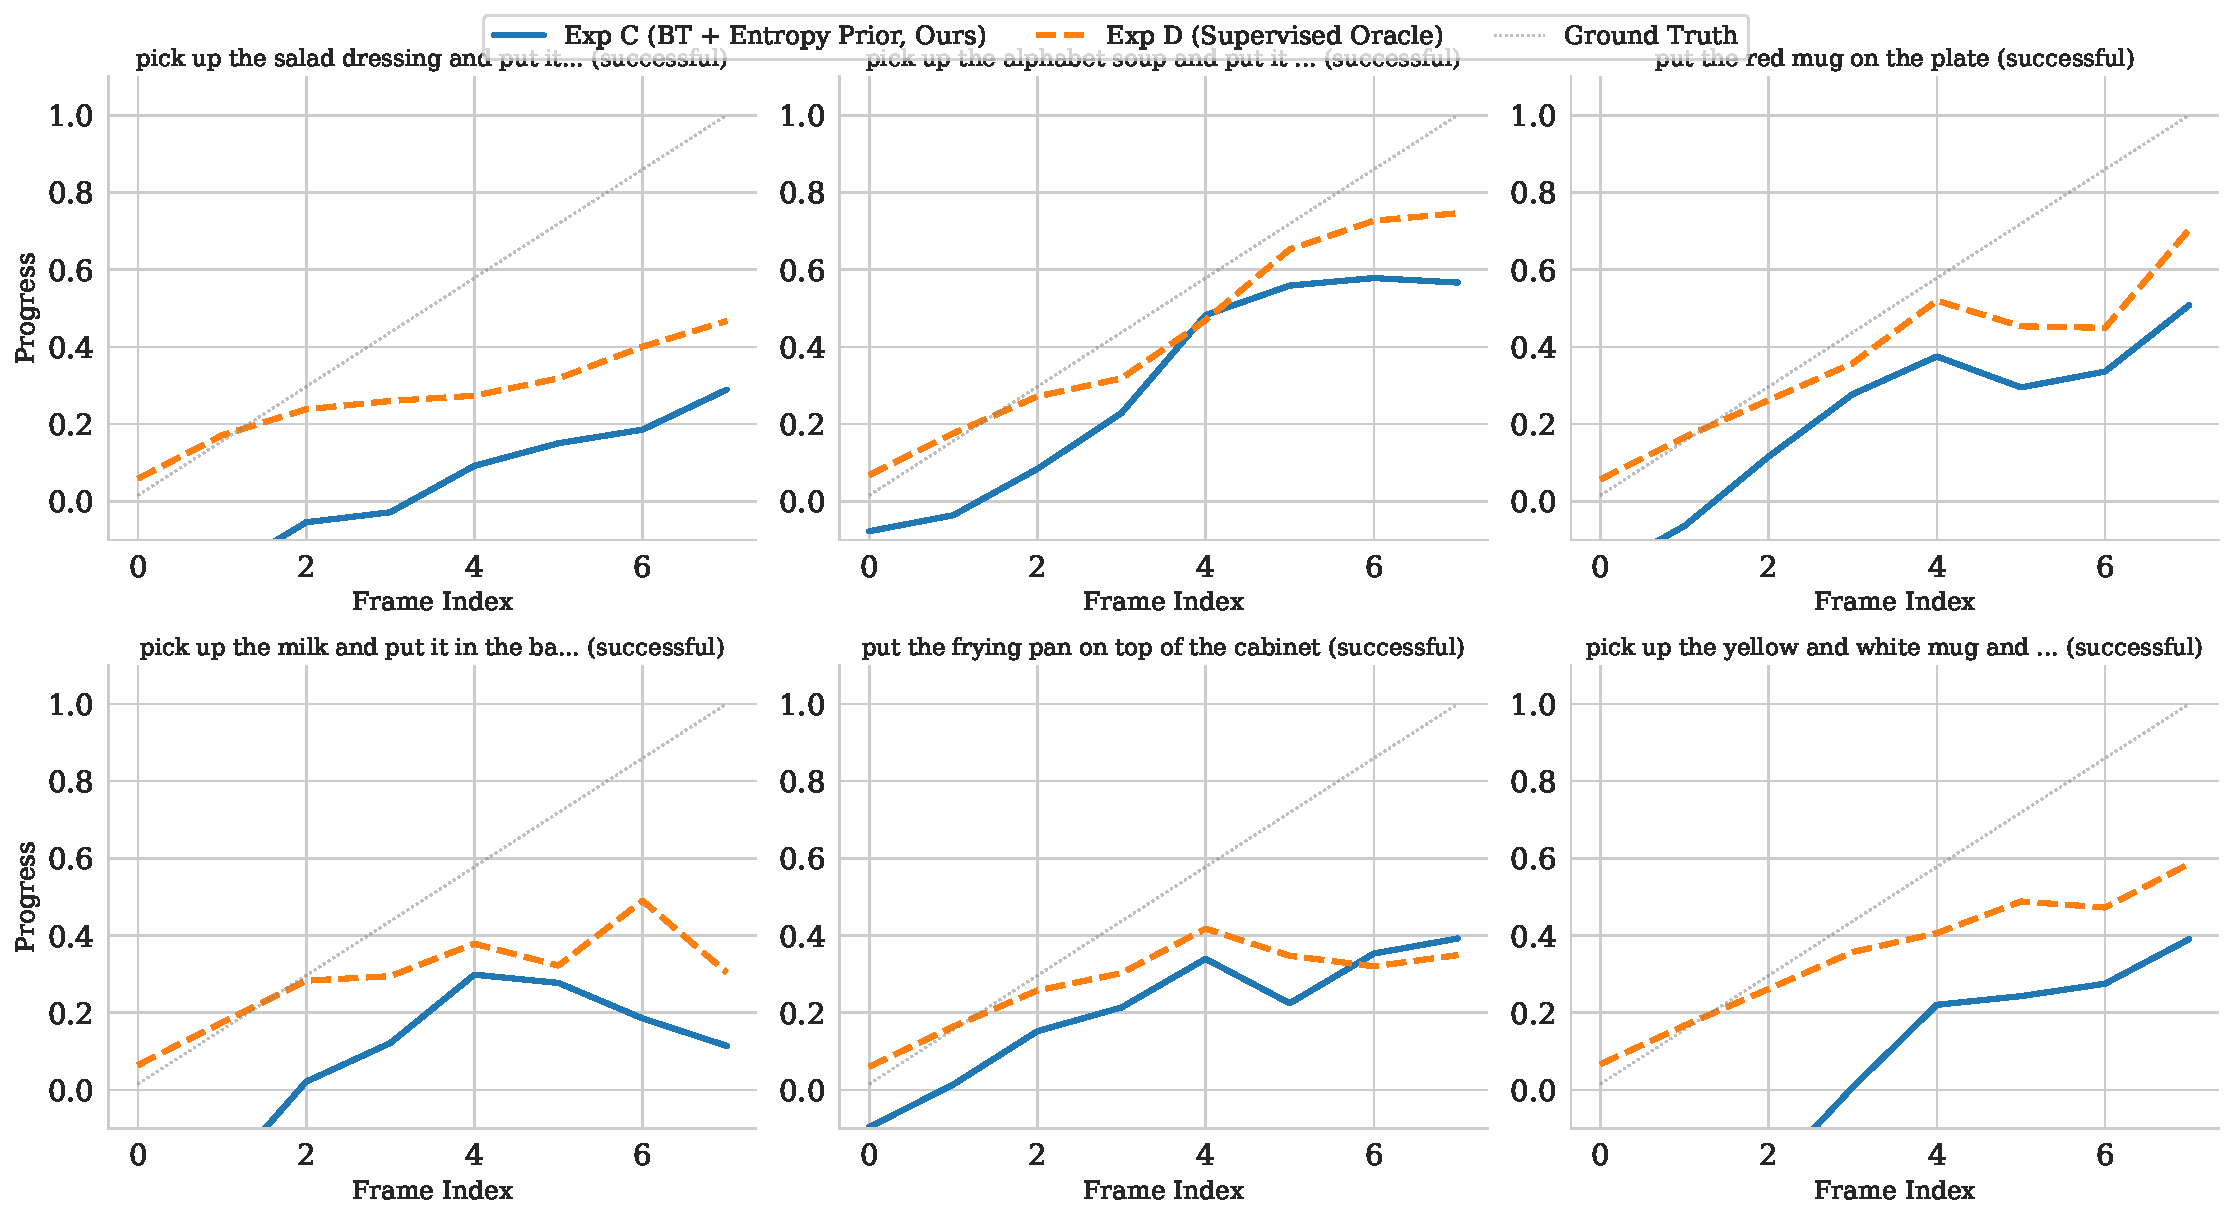
\includegraphics[width=0.95\textwidth]{figures/fig3_exp_c_vs_d_v2.pdf}
    \caption{同一批轨迹上本文方法（蓝色实线）与监督预言机（橙色虚线）的进度预测对比。灰色点线为真实时间步索引（线性进度基准）。本文方法的进度曲线与对角线高度吻合（VOC $r = 0.968$），对齐程度甚至优于使用帧级监督信号的预言机（VOC $r = 0.860$）。}
    \label{fig:exp_c_vs_d}
\end{figure}

\begin{figure}[htb]
    \centering
    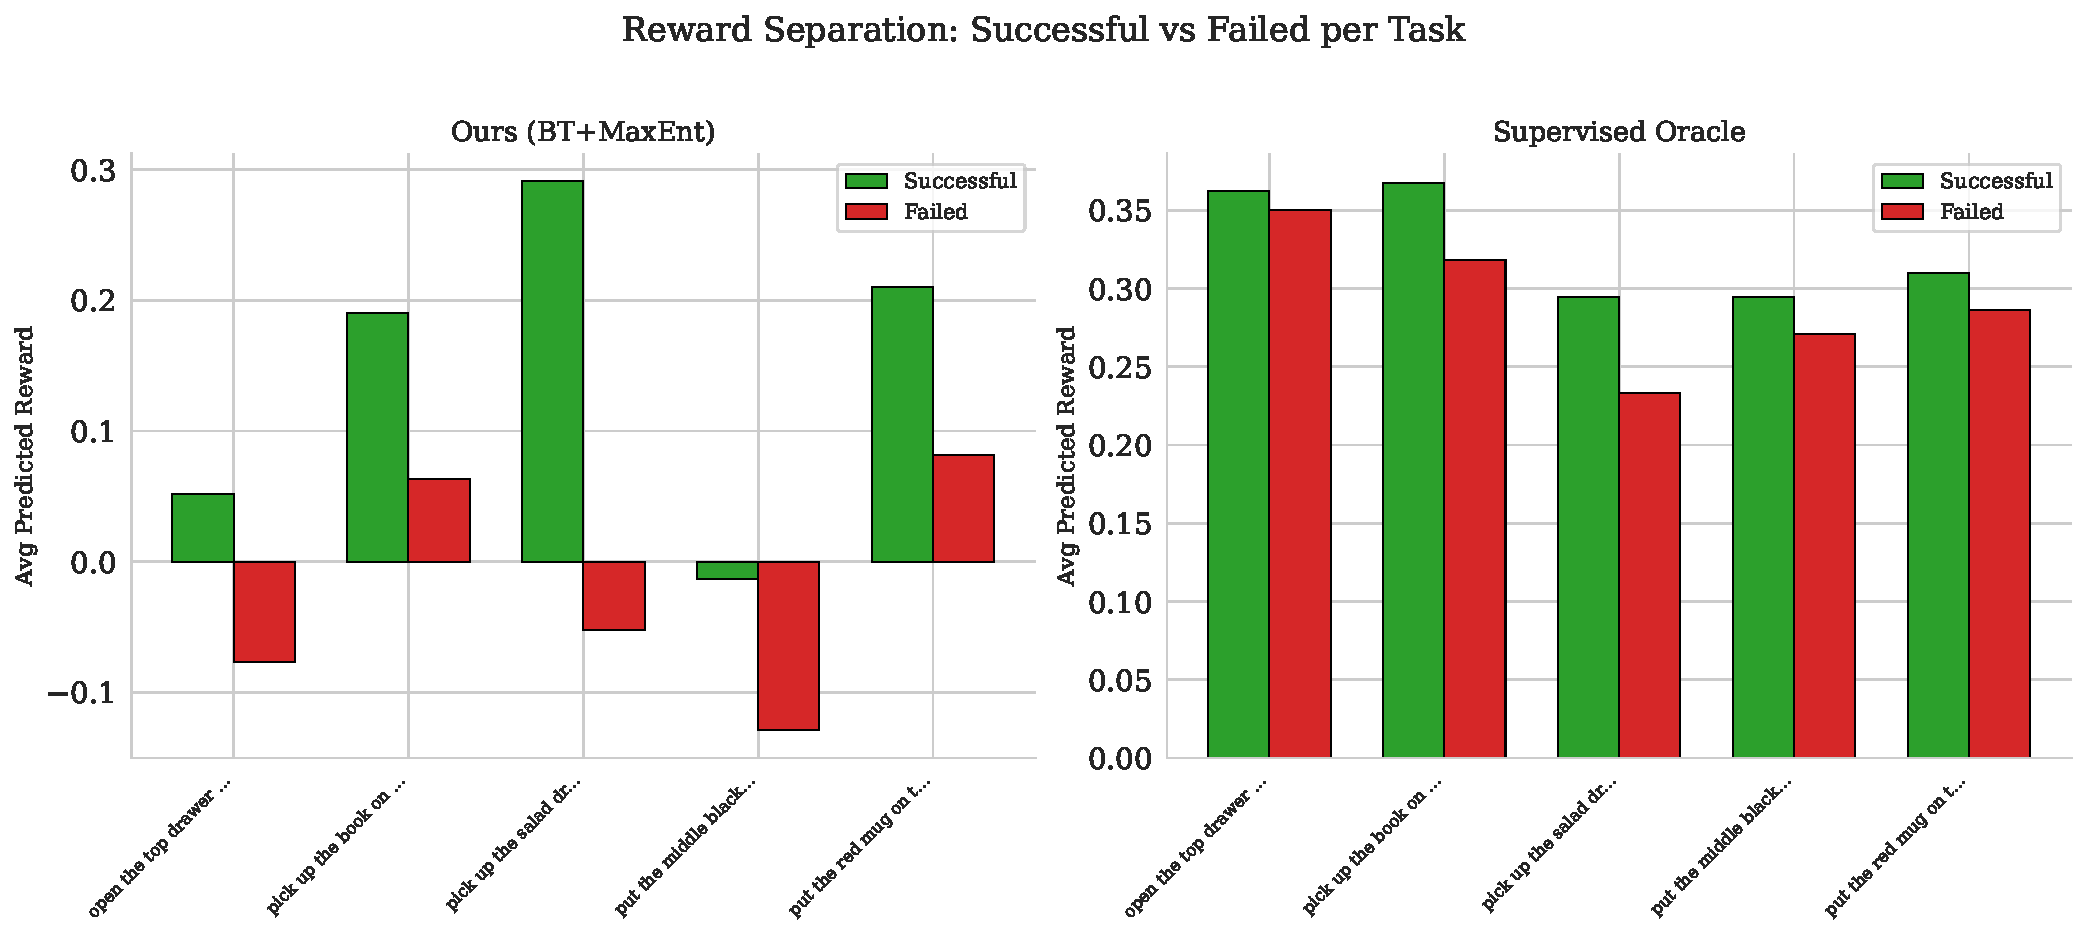
\includegraphics[width=0.95\textwidth]{figures/fig6_reward_separation_v3.pdf}
    \caption{本文方法与监督预言机在各任务上的奖励分离效果对比。绿色柱为成功轨迹的平均预测奖励，红色柱为失败轨迹。两种方法都能在所有任务上有效区分成败，但本文方法的分离幅度更大，说明其势函数为下游策略学习提供了更强的判别信号。}
    \label{fig:reward_separation}
\end{figure}

\subsection{分析}

\subsubsection{训练动态：避免梯度饱和}

将熵正则化直接应用于神经网络输出时，一个常见的陷阱是梯度饱和。我们的早期实验中，基于Softplus的朴素公式使得$\mathcal{L}_{struct}$在训练伊始就饱和于理论最大值（$T = 7$个增量时为$-\log 7 = -1.9459$），全程提供零梯度。两处关键改进解决了这个问题：
\begin{enumerate}[leftmargin=*,noitemsep]
    \item \textbf{从进度头中移除Sigmoid激活}，允许产生增量分布中足够方差的无界势值。
    \item \textbf{在Softmax归一化中引入温度参数}（$\tau = 0.1$），在计算熵之前放大增量之间的微小差异。
\end{enumerate}

\cref{tab:dynamics_qwen}和\cref{tab:dynamics_smol}分别展示了两种模型设置下的训练动态。

\begin{table}[ht]
    \centering
    \caption{$\mathcal{L}_{struct}$训练动态（Qwen3-VL-2B + LoRA，1250步）}
    \label{tab:dynamics_qwen}
    \makebox[\textwidth][c]{%
    \begin{tabular}{cccc}
    \toprule
    \textbf{步数} & $\mathcal{L}_{struct}$ & $\mathcal{L}_{BT}$ & $\sigma^2(\Delta\Phi)$ \\
    \midrule
    1 & $-1.003$ & 1.456 & 0.043 \\
    251 & $-1.167$ & 0.585 & --- \\
    501 & $-1.320$ & 0.594 & 0.029 \\
    651 & $-1.403$ & --- & --- \\
    951 & $-1.140$ & 0.423 & 0.036 \\
    \bottomrule
    \end{tabular}}
\end{table}

$\mathcal{L}_{struct}$在$-1.0$到$-1.4$之间波动，远离$-1.9459$的饱和点，梯度信号始终活跃。增量方差$\sigma^2(\Delta\Phi)$从$0.043$降至$0.029$--$0.036$，说明熵先验成功地推动了更均匀的增量分布。同时$\mathcal{L}_{BT}$正常收敛（$1.456 \to 0.423$），两个目标互不干扰。

\begin{table}[ht]
    \centering
    \caption{SmolVLM-500M完全微调下的训练动态（1000步）}
    \label{tab:dynamics_smol}
    \makebox[\textwidth][c]{%
    \begin{tabular}{ccc}
    \toprule
    \textbf{步数} & $\mathcal{L}_{struct}$ & $\mathcal{L}_{BT}$ \\
    \midrule
    10 & $-1.158$ & 0.905 \\
    100 & $-1.180$ & 0.655 \\
    500 & $-1.45 \sim -1.53$ & 0.121--0.178 \\
    1000 & $-1.55 \sim -1.56$ & 0.163--0.261 \\
    \bottomrule
    \end{tabular}}
\end{table}

SmolVLM-500M全参微调下也观察到相同的非饱和行为（\cref{tab:dynamics_smol}）：$\mathcal{L}_{struct}$从$-1.158$稳步下降至$-1.55$，$\mathcal{L}_{BT}$从$0.905$收敛至约$0.16$--$0.26$，与Qwen实验趋势一致。\cref{fig:training_dynamics}展示了完整的训练曲线。

\begin{figure}[htb]
    \centering
    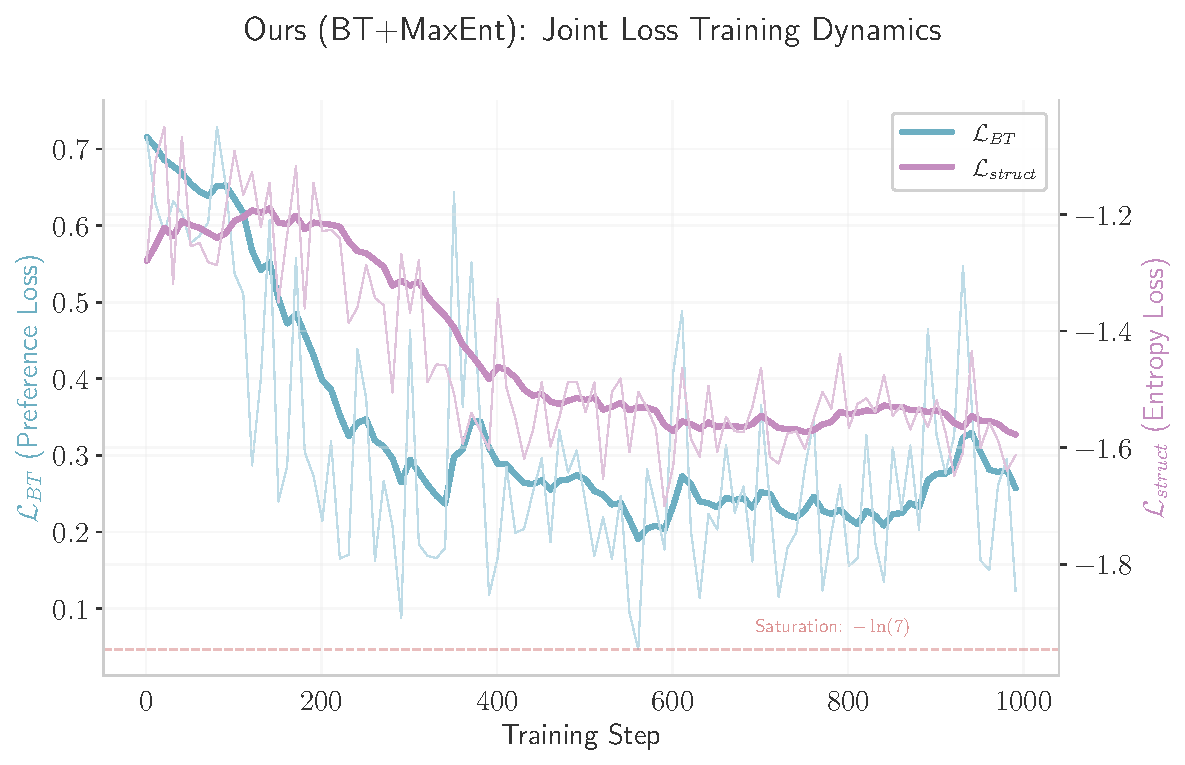
\includegraphics[width=0.95\textwidth]{figures/fig5_training_dynamics_v4_dual_axis.pdf}
    \caption{本文方法的联合训练动态（SmolVLM-500M全参微调）。蓝色曲线为偏好损失$\mathcal{L}_{BT}$（左轴），粉色曲线为结构损失$\mathcal{L}_{struct}$（右轴）。红色虚线标注了理论饱和点$-\ln 7 \approx -1.946$。$\mathcal{L}_{struct}$全程远离饱和点，梯度信号持续有效；$\mathcal{L}_{BT}$正常收敛，两个目标互不干扰。}
    \label{fig:training_dynamics}
\end{figure}

\begin{figure}[htb]
    \centering
    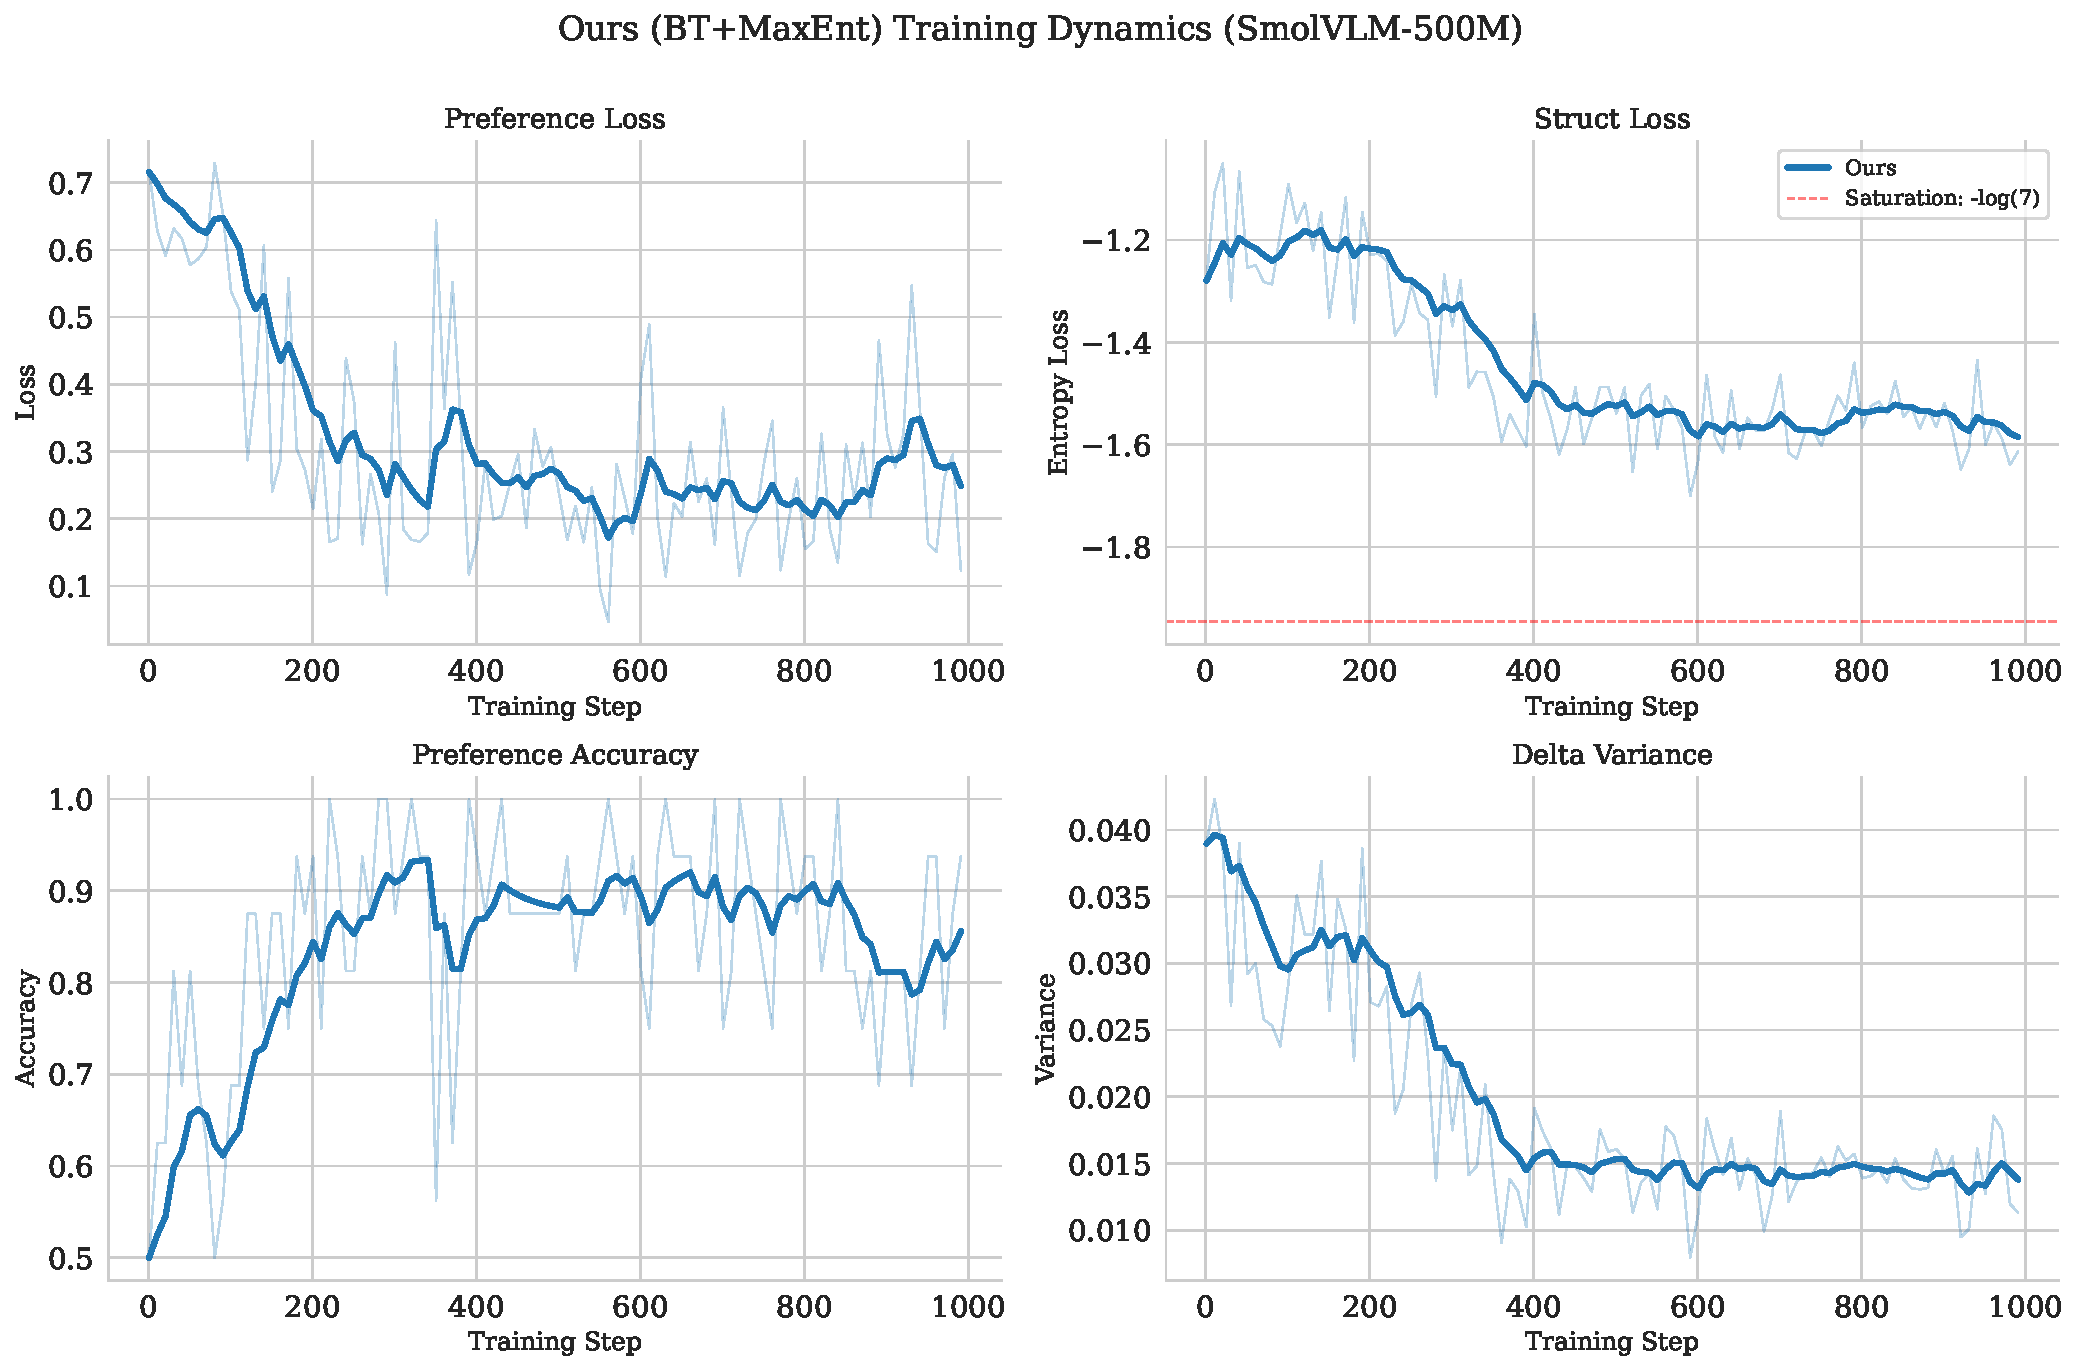
\includegraphics[width=0.95\textwidth]{figures/fig5_training_dynamics_v1.pdf}
    \caption{本文方法训练过程的四项关键指标：（左上）$\mathcal{L}_{BT}$持续收敛；（右上）$\mathcal{L}_{struct}$保持非饱和，梯度信号活跃；（左下）偏好预测准确率逐步提升至80\%以上；（右下）增量方差$\sigma^2(\Delta\Phi)$趋于稳定。}
    \label{fig:training_dynamics_detail}
\end{figure}

\subsubsection{方向歧义与$\mathcal{L}_{mono}$的作用}
\label{sec:direction}

移除Sigmoid激活后，势函数的方向变得不确定：它可能沿成功轨迹单调递减而非递增。这种歧义不影响轨迹级排序（BT比较对$\Phi$的全局符号不变），但会导致PBRS奖励信号方向反转。

$\mathcal{L}_{mono} = \text{mean}(\text{ReLU}(-\Delta\Phi_t))$通过惩罚负增量来解决这一问题。加入$\mathcal{L}_{mono}$后，本文方法在LIBERO-90上达到VOC $r = 0.968$，在LIBERO-10上达到$0.934$，均超过了监督预言机的$0.860$。作为对照，不使用方向约束的纯BT基线VOC $r$仅为$0.147$，L2平滑为$0.616$——方向约束对帧级对齐至关重要。

\subsubsection{定性分析：轨迹关键帧与进度曲线}

\cref{fig:trajectory_frames}展示了代表性轨迹的关键帧及本文方法的进度预测。成功轨迹（绿色）的进度曲线呈平稳上升趋势，反映出奖励模型对任务完成度的准确感知；失败轨迹（红色）的进度则停滞或偏低，符合预期。这种视觉化验证表明，$\mathcal{L}_{struct}$配合$\mathcal{L}_{mono}$不仅在统计指标上表现优异，其学习到的势函数在语义层面也是合理的。

\begin{figure}[htb]
    \centering
    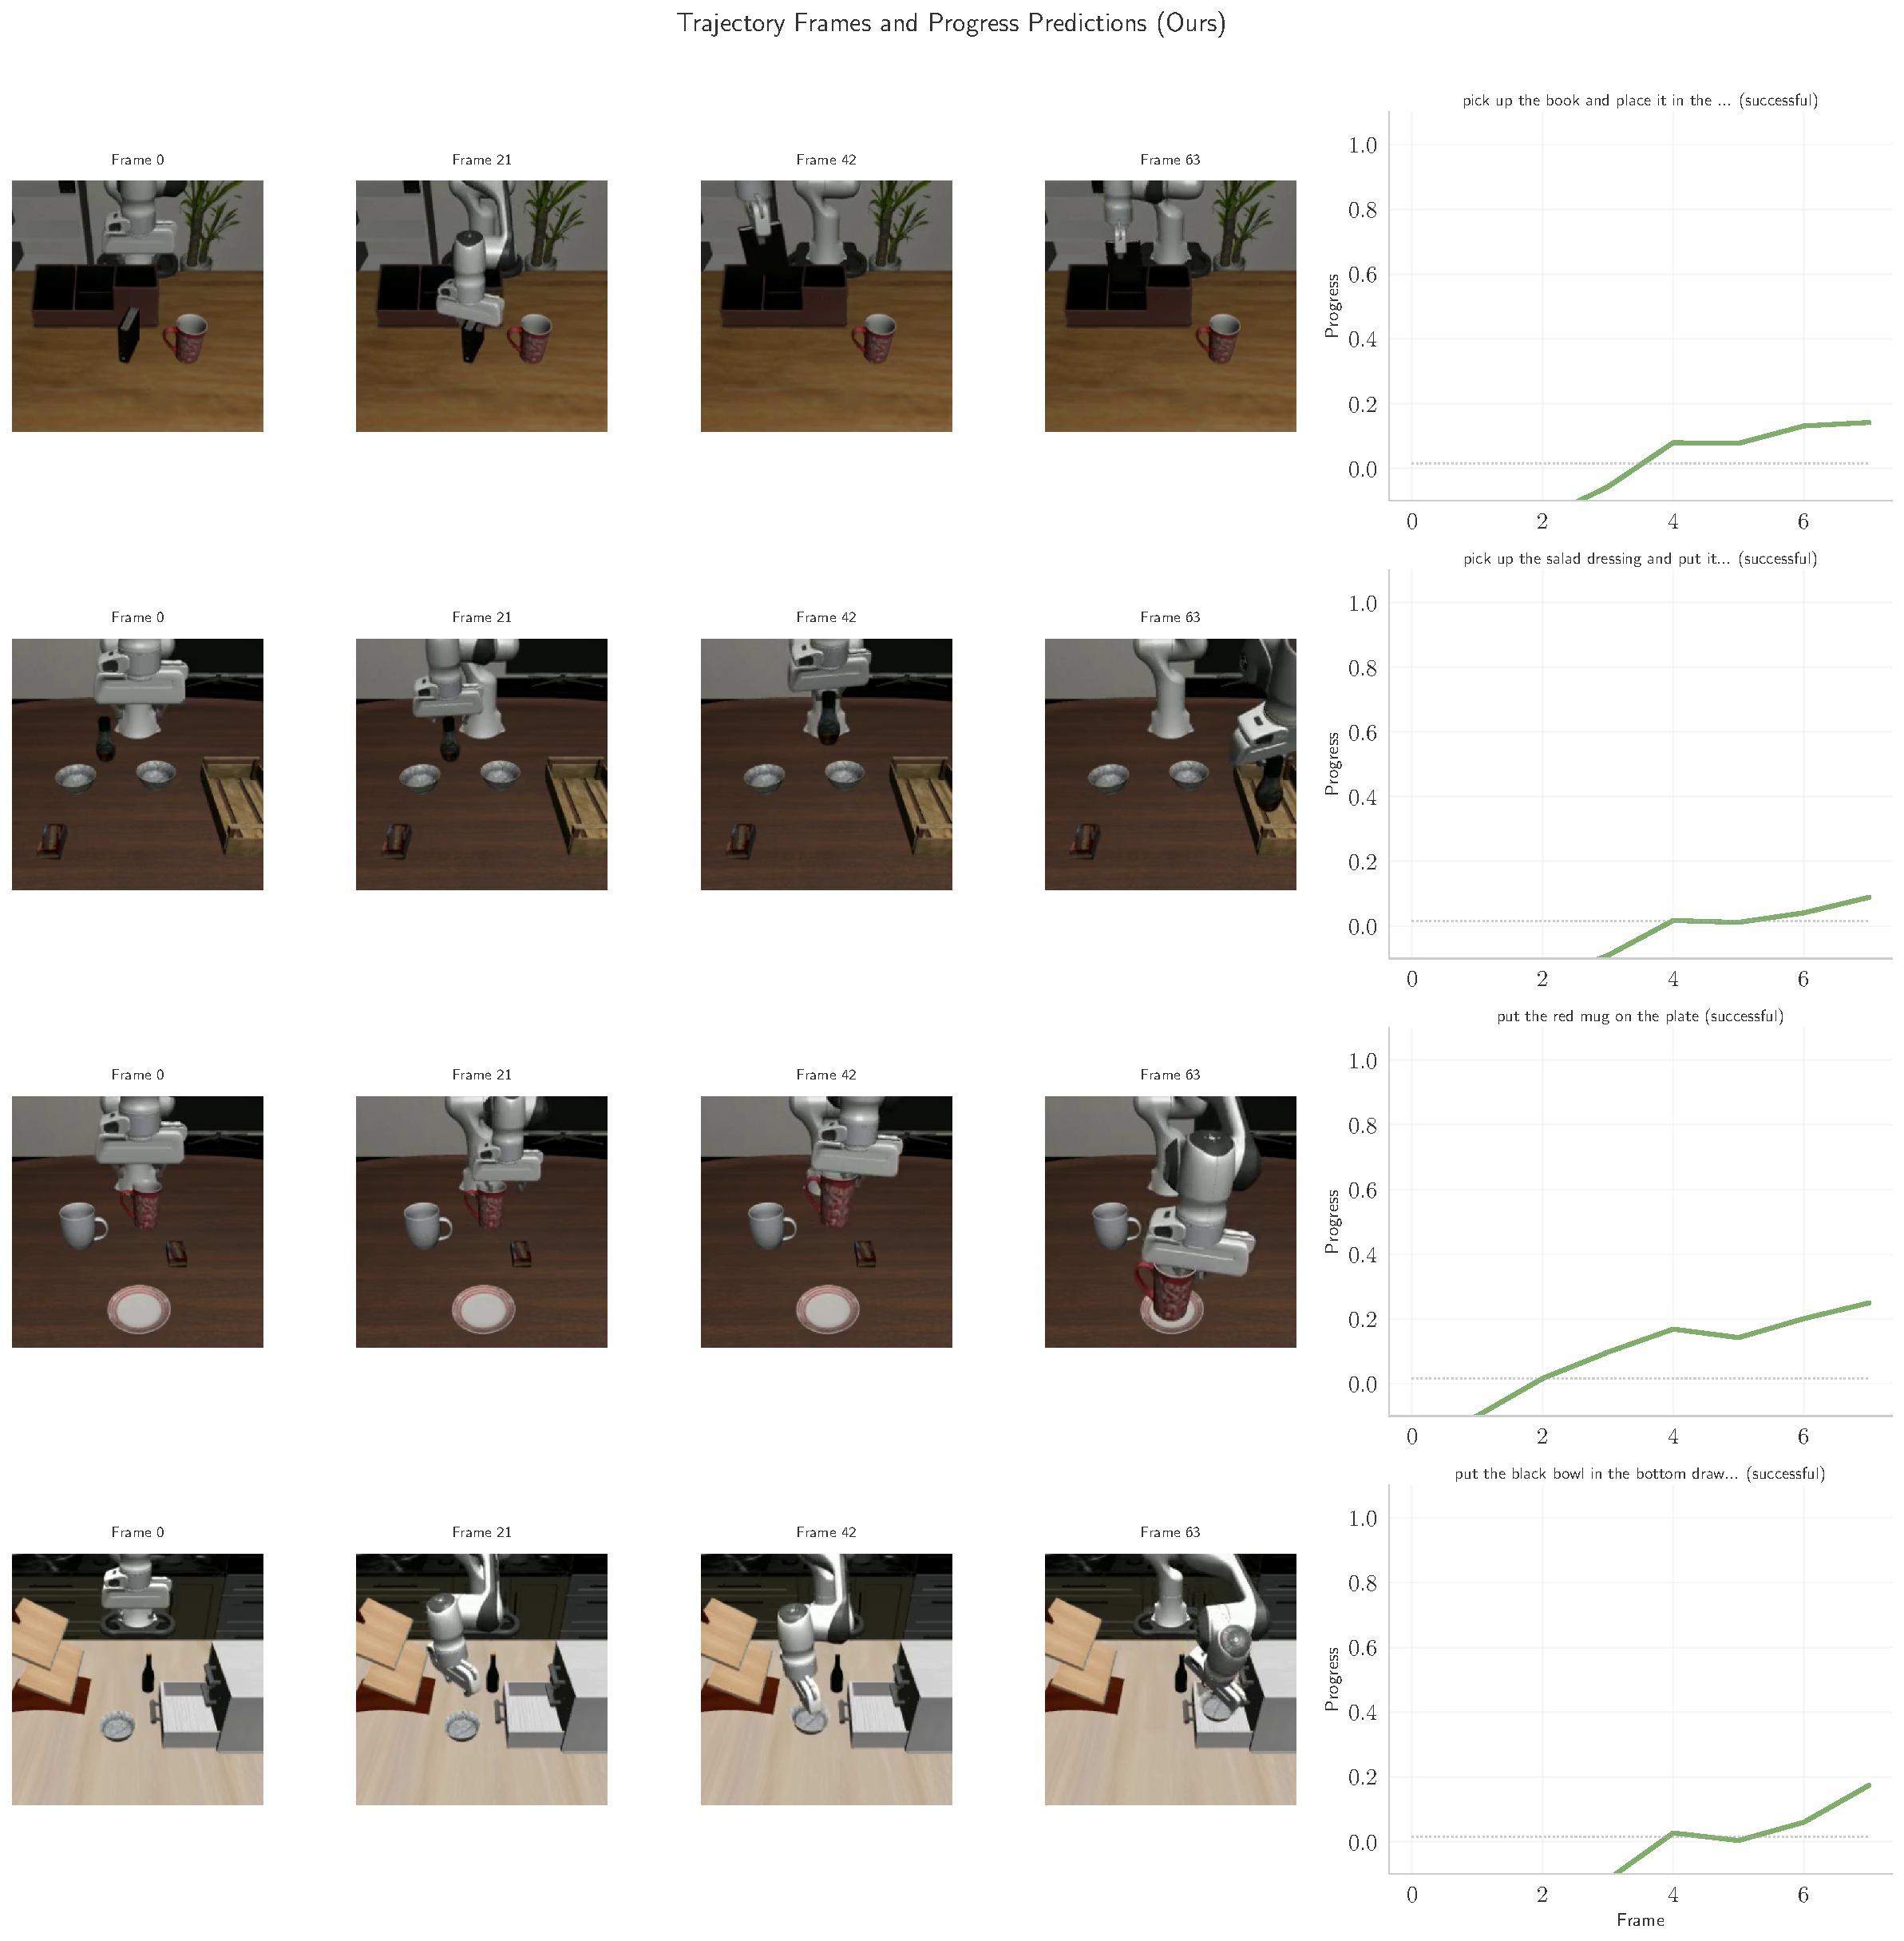
\includegraphics[width=0.95\textwidth]{figures/fig7_trajectory_frames_v1.pdf}
    \caption{代表性轨迹的关键帧与进度预测曲线。每行展示一条轨迹的四个等间距关键帧及本文方法的进度预测。成功轨迹（绿色）的进度平稳上升，失败轨迹（红色）的进度停滞或偏低，直观展示了奖励模型对任务完成度的感知能力。}
    \label{fig:trajectory_frames}
\end{figure}


\clearpage
\section{结论与展望}

本文揭示了基于偏好的奖励模型中一个此前被忽视的结构性问题——\textbf{单调性陷阱}：纯排序目标虽然能保证序数正确性，但无法约束PBRS部署所需的基数增量结构。为此，我们提出了最大熵增量先验（$\mathcal{L}_{struct}$），一种轻量的无监督正则化器，通过最大化时间增量分布的熵来规范势函数的曲率，配合单调性铰链损失$\mathcal{L}_{mono}$确保增量方向正确。

LIBERO基准上的四路消融实验清晰地展示了各组件的作用：纯BT基线的轨迹级排序尚可（Kendall $\tau = 0.680$），但帧级对齐严重失调（VOC $r = 0.147$）；L2平滑有所改善（$0.616$）但仍不充分；本文方法将VOC $r$推至$0.968$，在帧级对齐上超越了使用帧级监督信号的预言机（$0.860$，提升$12.6\%$），轨迹级排序也全面领先（Kendall $\tau$：$0.696$ vs $0.504$，提升$38.1\%$）。这一结果验证了核心论点：仅从序数偏好就能恢复对RL友好的基数增量结构，无需昂贵的帧级进度标注。

\textbf{未来工作。}当前实验在离线奖励模型评估指标上验证了方法的有效性。下一步将通过PBRS框架将训练好的势函数部署到在线RL循环中，使用SAC或PPO等策略优化算法在LIBERO环境中验证改善的增量结构能否转化为更高的任务成功率。此外，将方法推广到真实机器人平台和更大规模的VLM模型也是重要的研究方向。



\clearpage
\begin{thebibliography}{99}

\bibitem{christiano2017}
Christiano P F, Leike J, Brown T, Martic M, Legg S, Amodei D.
Deep reinforcement learning from human preferences[C].
Advances in Neural Information Processing Systems, 2017, 30.

\bibitem{lee2021}
Lee K, Smith L, Abbeel P.
PEBBLE: Feedback-efficient interactive reinforcement learning via relabeling experience and unsupervised pre-training[C].
Proceedings of the 38th International Conference on Machine Learning. PMLR, 2021, 139: 6152--6163.

\bibitem{brown2019}
Brown D S, Goo W, Nagarajan P, Niekum S.
Extrapolating beyond suboptimal demonstrations via inverse reinforcement learning from observations[C].
Proceedings of the 36th International Conference on Machine Learning. PMLR, 2019, 97: 783--792.

\bibitem{krack2026}
Krack P, Jülg T, Burgard W, Walter F.
Rewarding DINO: Predicting dense rewards with vision foundation models[J].
arXiv preprint arXiv:2603.16978, 2026.

\bibitem{ng1999}
Ng A Y, Harada D, Russell S.
Policy invariance under reward transformations: Theory and application to reward shaping[C].
Proceedings of the 16th International Conference on Machine Learning, 1999: 278--287.

\bibitem{liang2026}
Liang J, et al.
ROBOMETER: A vision-language model for robotic reward modeling via pairwise comparison and progress estimation[J].
arXiv preprint arXiv:2603.02115, 2026.

\bibitem{tan2026}
Tan S, et al.
Robo-Dopamine: Dense robotic reward via vision-language models[C].
Proceedings of the IEEE/CVF Conference on Computer Vision and Pattern Recognition, 2026.

\bibitem{ziebart2008}
Ziebart B D, Maas A L, Bagnell J A, Dey A K.
Maximum entropy inverse reinforcement learning[C].
Proceedings of the 23rd AAAI Conference on Artificial Intelligence, 2008: 1433--1438.

\bibitem{zhao2025}
Zhao Y, et al.
PrefMMT: Modeling human preferences in preference-based reinforcement learning with multimodal transformers[C].
Proceedings of the IEEE/RSJ International Conference on Intelligent Robots and Systems, 2025.

\bibitem{wiewiora2003}
Wiewiora E.
Potential-based shaping and Q-value initialization are equivalent[J].
Journal of Artificial Intelligence Research, 2003, 19: 205--208.

\bibitem{liu2023}
Liu B, Zhu Y, Gao C, Gupta A, Darrell T, Canny J, Stoica I, Finn C, Levine S.
LIBERO: Benchmarking knowledge transfer for lifelong robot learning[C].
Advances in Neural Information Processing Systems, 2023, 36.

\bibitem{bradley1952}
Bradley R A, Terry M E.
Rank analysis of incomplete block designs: I. The method of paired comparisons[J].
Biometrika, 1952, 39(3/4): 324--345.

\bibitem{shannon1948}
Shannon C E.
A mathematical theory of communication[J].
The Bell System Technical Journal, 1948, 27(3): 379--423; 27(4): 623--656.

\bibitem{jaynes1957}
Jaynes E T.
Information theory and statistical mechanics[J].
Physical Review, 1957, 106(4): 620--630.

\bibitem{sutton2018}
Sutton R S, Barto A G.
Reinforcement Learning: An Introduction[M].
2nd ed. Cambridge, MA: MIT Press, 2018.

\bibitem{schulman2017}
Schulman J, Wolski F, Dhariwal P, Radford A, Klimov O.
Proximal policy optimization algorithms[J].
arXiv preprint arXiv:1707.06347, 2017.

\bibitem{haarnoja2018}
Haarnoja T, Zhou A, Abbeel P, Levine S.
Soft actor-critic: Off-policy maximum entropy deep reinforcement learning with a stochastic actor[C].
Proceedings of the 35th International Conference on Machine Learning. PMLR, 2018, 80: 1861--1870.

\end{thebibliography}



\clearpage
\section*{致谢}

感谢指导老师在研究方向和论文写作上的悉心指导。感谢ROBOMETER\cite{liang2026}开源代码库为本工作提供的实验基础设施。本研究使用的计算资源由AutoDL云平台提供。


\end{document}
